% Chapter Template

\chapter{Analysis and Results - Active Monitoring} % Main chapter title

\label{Chapter6} % Change X to a consecutive number; for referencing this chapter elsewhere, use \ref{ChapterX}

\lhead{Chapter 6. \emph{Analysis and Results -  Active Monitoring}} % Change X to a consecutive number; this is for the header on each page - perhaps a shortened title

%----------------------------------------------------------------------------------------
%	SECTION 1
%----------------------------------------------------------------------------------------

%Trying to associate -> rejected some time -> status code = 12 ?
%Connecté et puis disconection abrupte -> code = 3 ?


\section{Analysis}
This chapter focuses on the active network analysis executed by the \texttt{OpenWrt} Linux probe. This device simulates a lambda user that tries to establish a connection with the UCL's wireless network in order to get an access to the Internet. The procedure followed by the \texttt{wpa\_supplicant} daemon is quite simple. A connection loop goes through all the networks specified in the program during the configuration phase, and then for each \texttt{SSID} several processes are executed. They can be grouped in three main steps.

\begin{enumerate}
\item Associate with the access point
\item Get an \texttt{IP} address
\item Check the availability of a set of services
\end{enumerate}

The goal here is to get an overview of the network infrastructure's performances from a user's point of view. This is really interesting since, most of the time, network administrators make their diagnosis only by focusing on the states of the components they directly manage. Here, we try to enhance these observations by adding the data collected with this new monitoring angle (i.e. the devices that use the network infrastructure).

The purpose of the active monitoring is, as mentioned before, to simulate a typical user's behavior on the network and make a bunch of tests in order to get a live overview of the current network status. During the connection loop, a various set of data is gathered and inserted into the log file. We have decided to focus on some key metrics. As a reminder, here are the information available into a typical log file (a full example is detailed in section \texttt{4.2.3.2}).

\begin{description}
	\item[Scan results]: The information concerning the set of access points located in the device's area as well as other \texttt{RF} related information.
	\item[AP tried]: The set of access points that the device tried to associate with.
	\item[AP connected]: The access point the supplicant connected with. Several access points can be found here since \texttt{wpa\_supplicant} has a roaming feature enabled by default and, by consequence, may decide to disconnect and reconnect to an access point with a better configuration.
	\item[Supplication Time]: Time elapsed during the connection establishment.
	\item [DHCP Time]: Time elapsed till an \texttt{IP} address is assigned to the device.
	\item [Services checks]: The results of the services availability and reachability tests.
\end{description}

After a defined amount of connections establishments on each \texttt{SSID}, the log file is sent to the server that is going to parse it and store the information accordingly in the database. These gathered data are then analysed by the server's threads. By aggregating those information throughout time, we can build an estimation of the overall quality experienced by the users when using the wireless network.

The following sections describe the analysis and conclusions we were able to make based on the information collected by the active probe after its deployment phase on the wireless network.


\section{Scanning}
As detailed above, the first part of the log file aggregates all the results received by the supplicant after having performed a network scan. Those information are quite interesting since they allow us to get live details about the current environment of the router. Thanks to those results we have a fully detailed overview of all the access points surrounding the it with information including their signal strengths, their frequencies and the \texttt{SSIDs} they broadcast.


\paragraph*{Current Wifi Environment} On the web platform, we can see the latest scan results sent by the device. This can help the administrators to diagnose some \emph{dead zones} on the campus. The results we have represent the exact surroundings of the router and by consequence we can directly tell if the area where the probe is located is correctly covered or not. 

We could have chosen to plot the signal strength throughout the day but in our situation the \texttt{RF} environment is quite stable and we prefer to provide the most recent scan results. Nevertheless, such analysis could be interesting for administrators that desire to monitor a room where the \texttt{RF} conditions significantly vary. All the data required are already available in the database to support that extension.

\paragraph*{Source} The source of those data is \texttt{wpa\_supplicant} itself. Before any association, the supplicant scans the environment to detect all the reachable access points. Those results come with the a bunch of related information. The following figure represents a typical scan result displayed on the web interface.

\begin{figure}[H]
	\centering
   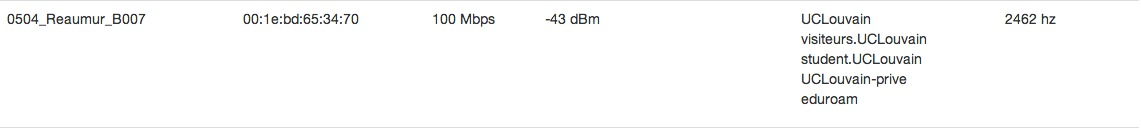
\includegraphics[width=1\textwidth]{Pictures/chapter6/scan-result.jpg}
   \caption{Example of a scan result}
\end{figure} 


\section{Access Points Interactions}
During the connection establishment phase, the supplicant makes several interactions with the access points. The first interaction it makes is in order to associate itself with one of the access points that broadcast the \texttt{SSID} of the network it tries to have get a connection to. The others concerns all the required data exchanges for the \texttt{802.1X} authentication process.

\subsection{Access Point Association}
The first thing the supplicant has to do in order to initiate a connection establishment is to associate itself with an access point. The algorithm used by the supplicant is quite straightforward. It lists all the access points that broadcast the \texttt{SSID} it wants to connect to in a decreasing order based on the signal strength. Then the supplicant tries to get associate with the first one. If the association is accepted by the AP, the authentication process is started and a connection with that particular AP is established. If the association is rejected, \texttt{wpa\_supplicant} tries with the second one, and so on. As an example, here is an association trace made by the supplicant in order to connect to \texttt{student.UCLouvain}.\\

\begin{lstlisting}[frame=single,breaklines=true,caption={Association trace for \texttt{student.UCLouvain}}]
Successfully initialized wpa_supplicant
wlan0: SME: Trying to authenticate with 00:1e:bd:65:34:71 (SSID='student.UCLouvain' freq=2437 MHz)
wlan0: Trying to associate with 00:1e:bd:65:34:71 (SSID='student.UCLouvain' freq=2437 MHz)
wlan0: CTRL-EVENT-ASSOC-REJECT bssid=00:1e:bd:65:34:71 status code=12
wlan0: SME: Trying to authenticate with 68:86:a7:1c:bb:11 (SSID='student.UCLouvain' freq=2462 MHz)
wlan0: Trying to associate with 68:86:a7:1c:bb:11 (SSID='student.UCLouvain' freq=2462 MHz)
wlan0: CTRL-EVENT-ASSOC-REJECT bssid=68:86:a7:1c:bb:11 status code=12
wlan0: SME: Trying to authenticate with 68:86:a7:30:a0:a1 (SSID='student.UCLouvain' freq=2412 MHz)
wlan0: Trying to associate with 68:86:a7:30:a0:a1 (SSID='student.UCLouvain' freq=2412 MHz)
wlan0: Associated with 68:86:a7:30:a0:a1
wlan0: CTRL-EVENT-EAP-STARTED EAP authentication started
wlan0: CTRL-EVENT-EAP-PROPOSED-METHOD vendor=0 method=4 -> NAK
wlan0: CTRL-EVENT-EAP-PROPOSED-METHOD vendor=0 method=21
wlan0: CTRL-EVENT-EAP-METHOD EAP vendor 0 method 21 (TTLS) selected
wlan0: CTRL-EVENT-EAP-SUCCESS EAP authentication completed successfully
wlan0: WPA: Key negotiation completed with 68:86:a7:30:a0:a1 [PTK=CCMP GTK=TKIP]
wlan0: CTRL-EVENT-CONNECTED - Connection to 68:86:a7:30:a0:a1 completed (auth) [id=0 id_str=]
\end{lstlisting}

Notice that, during the authentication process, the \texttt{EAP-PROPOSED-METHOD} with value equals \textit{4} stands for the \texttt{EAP-MD5} method, which is rejected by the controller.


\paragraph*{Rejection} The first observation we made regarding the association interactions was that our device does not always connect with the best access point in terms of signal strength. Indeed, as explained above, \texttt{wpa\_supplicant} lists all the APs it might connect with in a decreasing order based on that signal strength. But as we can see on the example with the association trace for \texttt{student.UCLouvain}, sometimes the association is rejected by the access point, forcing the supplicant to try other APs until the association is finally accepted. This is an issue since the device might be associated with an access point with a lower signal than the others.

During our investigations we have noticed that each time an association is rejected, the status code is always equal to \textit{12}. By looking into the \texttt{wpa\_supplicant} source code\footnote{src/common/ieee802\_11\_defs.h} we have found that this status code refers to \texttt{WLAN\_STATUS\_ASSOC\_DENIED\_UNSPEC} that states for \emph{Access Denied Unspecified}. Despite the fact that our monitoring tool was able to detect this issue by analysing all the events sent from the supplicant, a deeper debugging on the access point and the controller is required in order to find the precise cause. Since we do not have a direct access to the APs nor the controller this debugging is outside the scope of our system. Nevertheless, we record all the access points \texttt{BSSID} the supplicant tried to associate with and we are able to provide the quantity of APs that has rejected the association request.With that metric, and by crossing it with the scan results, we are able to tell where the issue occurred.


\paragraph*{Disconnection} Another issue we noticed during our analysis is the fact that the device sometimes disconnects from the AP and reconnects, to the same AP or to another one, forcing the daemon to restart the associate and authentication process. This behavior can be interpreted as roaming but it is quite disturbing when performing our tests. Like before, we have recorded all the events generated by the supplicant and identified the cause. In the case of \texttt{CTRL-EVENT-DISCONNECTED} event, two reasons have been noticed. The first, \textit{reason=3} meaning that the AP went offline and is deauthenticating the client. The second, \textit{reason=4} that refers to the fact the deauthentication is due to inactivity (i.e. client session timeout exceeded). The following listing continues the example aboves and shows a disconnection event.\\

\begin{lstlisting}[frame=single,breaklines=true,caption={Example of Deconnection trace}]
wlan0: CTRL-EVENT-CONNECTED - Connection to 68:86:a7:30:a0:a1 completed (auth) [id=0 id_str=]
wlan0: CTRL-EVENT-DISCONNECTED bssid=68:86:a7:30:a0:a1 reason=4 locally_generated=1
wlan0: SME: Trying to authenticate with 68:86:a7:1c:d0:61 (SSID='student.UCLouvain' freq=2412 MHz)
wlan0: Trying to associate with 68:86:a7:1c:d0:61 (SSID='student.UCLouvain' freq=2412 MHz)
wlan0: CTRL-EVENT-EAP-STARTED EAP authentication started
wlan0: CTRL-EVENT-EAP-PROPOSED-METHOD vendor=0 method=4 -> NAK
wlan0: CTRL-EVENT-EAP-PROPOSED-METHOD vendor=0 method=21
wlan0: CTRL-EVENT-EAP-METHOD EAP vendor 0 method 21 (TTLS) selected
wlan0: CTRL-EVENT-EAP-SUCCESS EAP authentication completed successfully
wlan0: WPA: Key negotiation completed with 68:86:a7:1c:d0:61 [PTK=CCMP GTK=TKIP]
wlan0: CTRL-EVENT-CONNECTED - Connection to 68:86:a7:1c:d0:61 completed (auth) [id=0 id_str=]
\end{lstlisting}

Here again, if such issue wants to be properly diagnosed, deeper access to the infrastructure is required. For now, our application monitors the amount of reconnections that happened during the test phases. We plot that information as well as the number of associations tried for each \texttt{SSID}. The following figure shows such a graph for the \texttt{student.UCLouvain} network.

\begin{figure}[H]
	\centering
   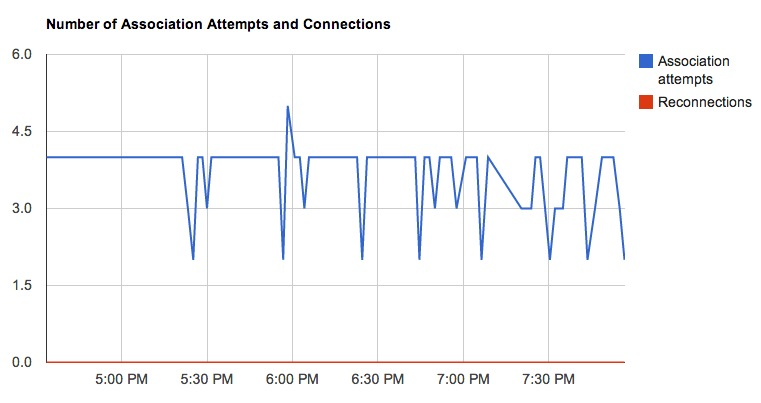
\includegraphics[width=1\textwidth]{Pictures/chapter6/ap-interactions.jpg}
   \caption{Number of associations and reconnections}
\end{figure} 

We can see on that figure that there were not any reconnections during the deployment. In fact, that is not exactly true. Indeed, we have noticed some reconnections, thanks to the the \texttt{wpa\_supplicant} events, but each time the supplicant disassociated itself with the AP it directly reassociated with the same AP. This is not represented on the graph because we have chosen to only display the reconnections to different APs and not to the same one. Regarding the associations we can see that they vary from one to five APs maximum with the most frequently occurring value being four access points.

\paragraph*{Source} All these logs are generated by \texttt{wpa\_supplicant} and provided through an event generator mechanism. Our program is interfaced with the supplicant and is able to record all those events, parse them and insert useful information into our own log file. These events provide a rich source of information since they trace everything that is happening between the supplicant and the network components.


\section{Time Durations}
Time is an important factor when dealing with wireless networks performances. Indeed, the users can be really annoyed when the duration taken for a connection establishment begins to take too much time. We have decided to keep track of the time duration it takes for \texttt{wpa\_supplicant} to establish a connection with the network. Concretely, we start a timer when the command \texttt{SELECT\_NETWORK} is sent to the control interface to start the connection phase and we stop it as soon as a \texttt{WPA-EVENT-CONNECTED} event is received. We also keep track of the time it takes for the \texttt{DHCP} servers to provide an \texttt{IP} address to the supplicant. The methodology is the same as the one used for the connection establishment's duration computation. A timer is started as soon as the device is connected to the network and before it sends a \texttt{DISCOVER} message to the \texttt{DHCP} servers, and is stopped as soon as a lease for an \texttt{IP} address is obtained. 

\paragraph*{Decomposition} An interesting feature of this analysis is that, as we just mentioned, we can decompose the waiting time of the users in different parts. By observing the proportion of each part, we can point out what part constitutes the bottleneck of the connection establishment. Since we gathered those indicators during our deployment phase, we are able to monitor their evolution and make the distinction between persistent problems and the isolated cases. By plotting the data from both parts on a same graph we are able to depict the evolution of the connection establishment duration through time for each \texttt{SSID}. The following two figures represent the time taken by \texttt{wpa\_supplicant} and by the \texttt{DHCP} servers during the deployment.

\begin{figure}[H]
	\centering
   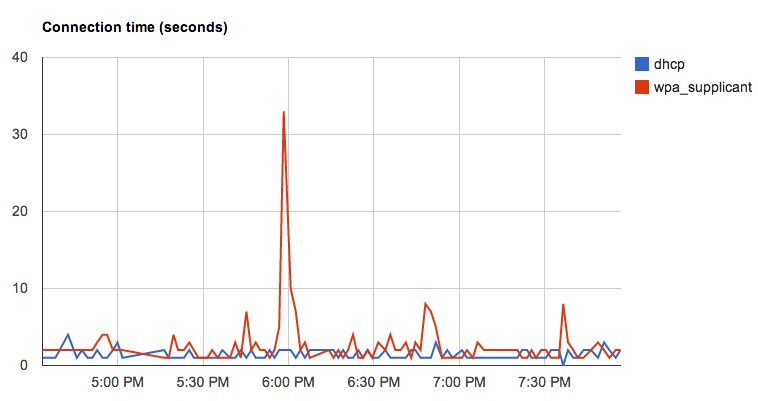
\includegraphics[width=1\textwidth]{Pictures/chapter6/time-student.jpg}
   \caption{Connection time for \texttt{student.UCLouvain}}
\end{figure} 

\begin{figure}[H]
	\centering
   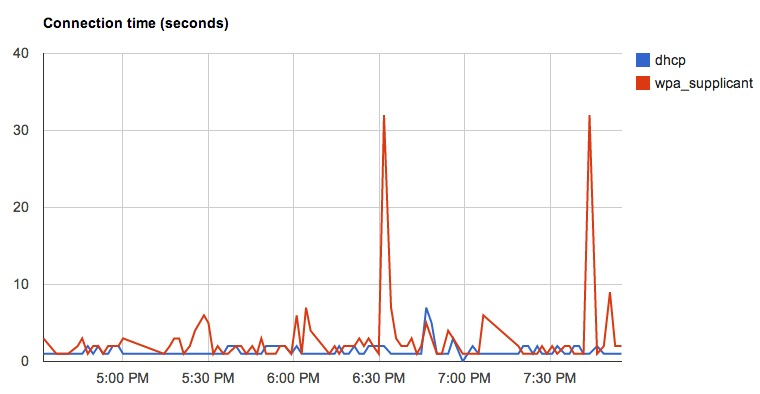
\includegraphics[width=1\textwidth]{Pictures/chapter6/time-eduroam.jpg}
   \caption{Connection time for \texttt{eduroam}}
\end{figure} 

We can see that the time taken by \texttt{wpa\_supplicant} and by the \texttt{DHCP} servers are totally different. The \texttt{DHCP} servers took only four seconds maximum to assign an \texttt{IP} address to the device in the \texttt{student.UCLouvain} network and up to seven seconds maximum in the \texttt{eduroam} network. Since those maximum values only occur from time to time we can safely affirm that the \texttt{DHCP} servers do not have any implications in the connection establishment bottleneck. On the other side, \texttt{wpa\_supplicant} seems to be more unstable and can experience peaks up to thirty seconds in order to get a connection. 

\paragraph*{Peaks} We have investigated on the possible reasons of those peaks and we have noticed that \texttt{wpa\_supplicant} seems to spend a lot of time in the association phase. As said before, the AP is sometimes rejecting the device and, thus, forces the supplicant to associate to other ones. This may induce some latency in the connection phase and impact on perceived performance of the user. If we compare the graph about the number of associations and reconnections for the \texttt{student.UCLouvain} network with the connection time graph for the same network we can see that most of the time the peaks coincide with the number of connection attempts. 

\begin{figure}[H]
	\centering
   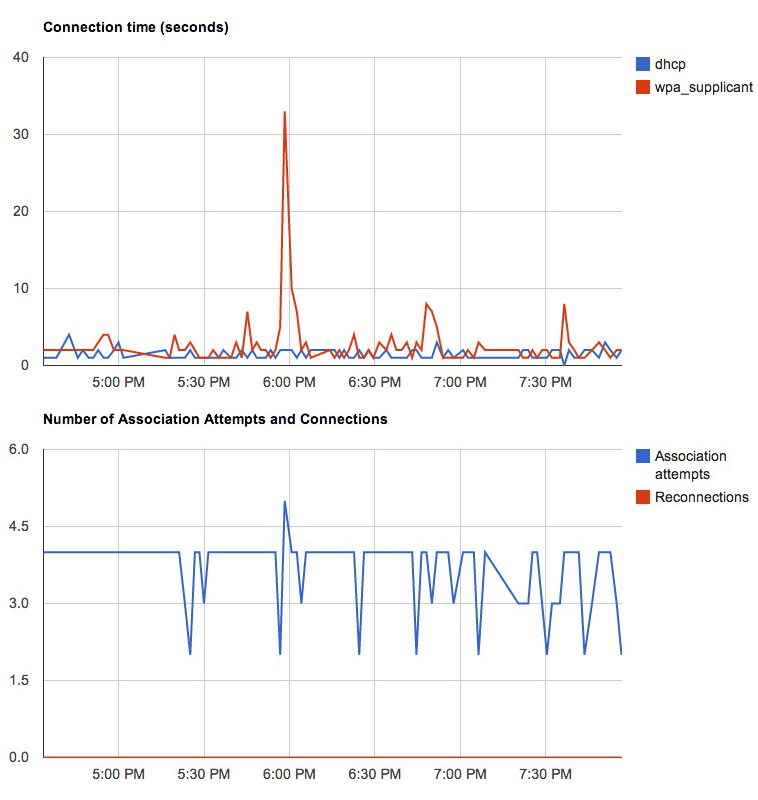
\includegraphics[width=1\textwidth]{Pictures/chapter6/time-explain.jpg}
   \caption{Comparison between time duration and associations-reconnections in the \texttt{student.UCLouvain} network}
\end{figure} 

In order to understand why those rejected associations happen, we also examined the log file of the \texttt{WiSM} available on the \texttt{Octopussy} platform \cite{octopussy} and we found a lot of the same \texttt{LWAPP} error message.\\

\begin{lstlisting}[frame=single,breaklines=true,caption={\texttt{WiSM} association error message}]
*apfReceiveTask: Jul 18 18:22:01.632: %LWAPP-3-INVALID_AID2: spam_api.c:1226 Association identifier 8 for client cc:52:af:7f:d8:8b is already in use by cc:52:af:7f:d2:1
\end{lstlisting}

The explanation\footnote{http://www.cisco.com/c/en/us/td/docs/wireless/controller/message/guide/controller\_smg/msgs6.html} \texttt{Cisco} gives for that error message is that an internal error caused an invalid association ID to be received from an AP for the indicated client and that the client may experience some communications problems. This seems to be related to duplicate and invalid association identifier entries for \texttt{FlexConnect} clients. \texttt{Cisco FlexConnect} is a technology that allows APs to be remotely deployed from the controller but allow for distributed switching of local packets. A local \texttt{VLAN ID} from the AP's switch is mapped to an \texttt{SSID} instead of tunneling all the traffic back to the \texttt{WLAN} controller to be switched centrally. This error message can also be observed for several devices on the network an unfortunately, according to \texttt{Cisco}, no work around is possible for that kind of error.


\paragraph*{Source} This analysis heavily uses the event mechanism of \texttt{wpa\_supplicant} to generate those estimations of duration. We complete the analysis with the controller logs that are available on the \emph{Gathering} part. This is also a good example that a system embedding all the monitoring tools can help generating better analysis about issues on a complex infrastructure.


\section{Services Availability}
We want our application to be able to give a performance and quality overview of the network every time a new connection is established. In order to provide that kind of information we have designed a special services reachability and availability test for a given selection of services. As mentioned in section \texttt{4.2.3.2}, we have divided our test into two parts. First we perform a \texttt{DNS} query on the two UCL's \texttt{DNS} servers to make sure that both servers are reachable. Then we test the \texttt{TCP} connection to the main UCL's services added to the collection of the ten most visited website in the world using simple \texttt{socket} connections. The resulting data is inserted into the log file that is forwarded to the server. After having received several log files from the router we were able to check the results and make some analysis on them. By decoupling those analysis, we can localize more precisely the connectivity issues. The following figure shows how the data concerning the services is represented on the web platform.

\begin{figure}[H]
	\centering
   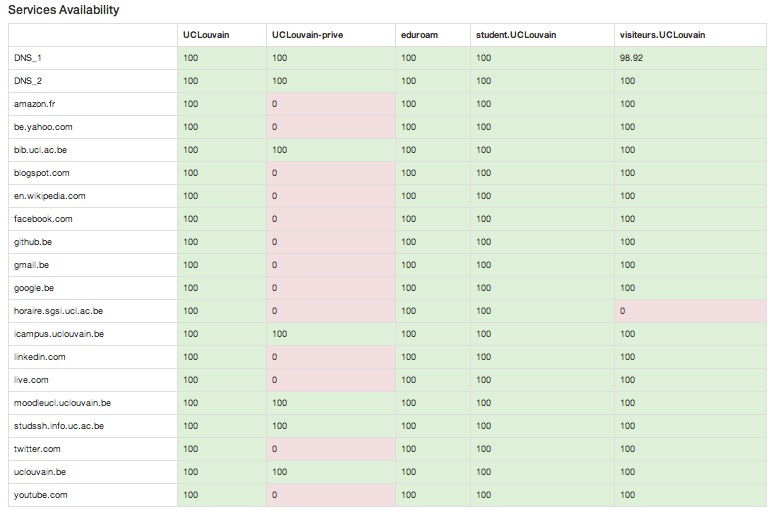
\includegraphics[width=1\textwidth]{Pictures/chapter6/services.jpg}
   \caption{Services availability on the UCL network}
\end{figure} 


\paragraph*{DNS} The first conclusion we made after analysing the results is that both \texttt{DNS} servers are always reachable and accessible within the five \texttt{VLANs}. Still, we noticed that during the deployment we had a reachability rate of 98.92 percent for the first server with the \texttt{visiteurs.UCLouvain} network. This is not an issue since the second server, that had rate of 100 percent, backs up the first one if a connectivity issue arise between that server and the users. Addresses are always resolved.

\paragraph*{Services test} The results of the service reachability tests depend on which network the test is executed on. Indeed, the UCL's wireless documentation states that some \texttt{VLANs} restrict the range of accessible websites. We were able to confirm that information thanks to these tests. Upon our analysis we can see that, only two networks have some restrictions.

\begin{itemize}
	\item [-] \texttt{UCLouvain-prive}
	\item [-] \texttt{visiteurs.UCLouvain}
\end{itemize}

For the first one, all the services that are not related to the UCL are forbidden. Indeed, this network is only for accessing the UCL wireless configuration page and others such as \texttt{www.icampus.uclouvain.be} or \texttt{www.bib.ucl.ac.be}.

For the second one, all the services are reachable except \texttt{horaire.sgsi.ucl.ac.be}. This is because the port used to access this website is \texttt{8080} and this port has been blocked by the firewall on that \texttt{VLAN} as well as for \texttt{UCLouvain-prive}.

By checking periodically those services, we can generate their availability rate which can be a good indicator to determine the network's performance experienced by the user.


\paragraph*{Source} The data used in this analysis are completely generated by our system. The tests are performed by subroutines implemented in our \texttt{C} program. All the information are centralized in the server that also handles all the data aggregating and analysis phase.

%\section{Limitations}
%During the development 

%The main limitation of those analysis is the interface of \texttt{wpa\_supplicant}. We interface our program with it and use its message and functions to generate our data. A more powerful approach would be to work directly in the \texttt{wpa\_supplicant} code and extend it with our program. That is far more complex and would require a lot more of time. Nevertheless, it is really an interesting idea for future extensions for our system.

\section{Summary}
In this chapter, information about the analysis performed by our active monitoring program has been developed. Thanks to all the collected data plotted into graphs we were able to spot some issues on the network that we tried to understand and describe. The active tool is still a prototype but, as we have seen throughout this chapter, it can help diagnose the network with a different view since the information it is able to gather is not always reported in the controller log files.
